\documentclass[border=4pt]{standalone}
\usepackage{amsmath}
\usepackage{tikz}
\usetikzlibrary{shapes.geometric,arrows.meta,positioning,fit}
\begin{document}
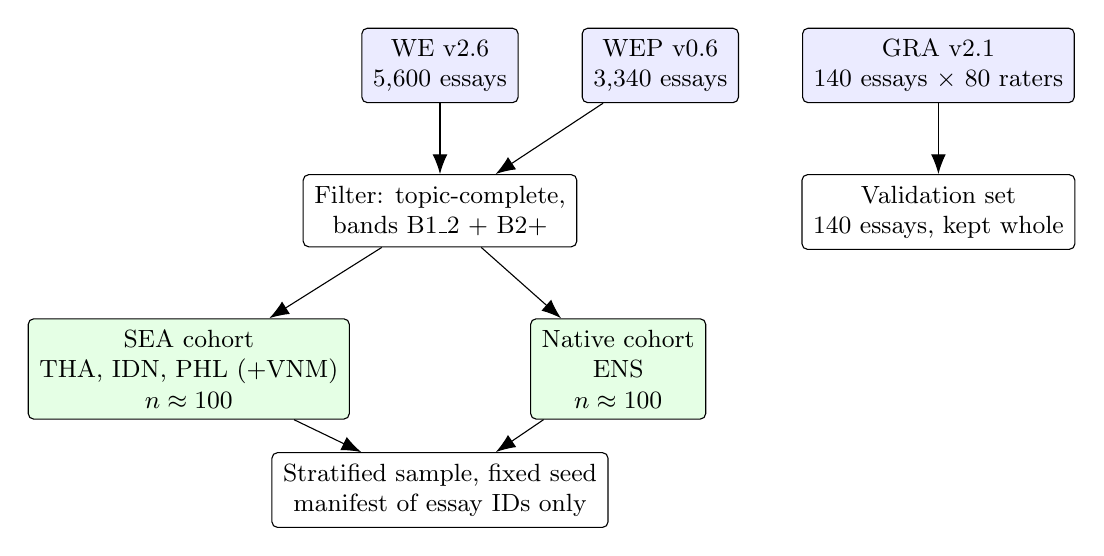
\begin{tikzpicture}[
  node distance=5mm and 8mm,
  box/.style={rectangle, rounded corners=2pt, draw, align=center,
              minimum height=8mm, inner sep=4pt, font=\small},
  mod/.style={box, fill=blue!8},
  coh/.style={box, fill=green!10},
  arr/.style={-{Latex[length=2.5mm]}}]
  \node[mod] (we) {WE v2.6\\5{,}600 essays};
  \node[mod, right=of we] (wep) {WEP v0.6\\3{,}340 essays};
  \node[mod, right=of wep] (gra) {GRA v2.1\\140 essays $\times$ 80 raters};
  \node[box, below=9mm of we] (filter) {Filter: topic-complete,\\bands B1\_2 + B2+};
  \node[coh, below left=9mm and -6mm of filter] (sea) {SEA cohort\\THA, IDN, PHL (+VNM)\\$n \approx 100$};
  \node[coh, below right=9mm and -6mm of filter] (ens) {Native cohort\\ENS\\$n \approx 100$};
  \node[box, below=9mm of gra] (val) {Validation set\\140 essays, kept whole};
  \node[box, below=26mm of filter] (sample) {Stratified sample, fixed seed\\manifest of essay IDs only};
  \draw[arr] (we) -- (filter);
  \draw[arr] (wep) -- (filter);
  \draw[arr] (filter) -- (sea);
  \draw[arr] (filter) -- (ens);
  \draw[arr] (sea) -- (sample);
  \draw[arr] (ens) -- (sample);
  \draw[arr] (gra) -- (val);
\end{tikzpicture}
\end{document}
